\documentclass[11pt]{article}

%% Imports as the graphics functions and color options
\usepackage{graphicx,color}
\usepackage{setspace}
\usepackage{subfig}
\usepackage{listings}
\usepackage{algorithmic}
\usepackage{algorithm}
\usepackage{comment}

% Use Times Roman font 
\usepackage{mathptmx}
\renewcommand{\rmdefault}{ptm}


%% Make the margins 1 inch all around
\setlength{\textheight}{9.25in}
\setlength{\topmargin}{-0.75in}
\setlength{\textwidth}{7.0in}
\setlength{\oddsidemargin}{-0.25in}
\setlength{\evensidemargin}{-0.25in}

%% This enables the figure to use the same font family as the document
%% (i.e., font family and size is the same in the figure as it is
%% in the text).
\gdef\SetFigFont#1#2#3#4#5{}

%% \figref is used to make all figure references consistent and easy to change
\newcommand{\figref}[1]{Figure~\ref{#1}}
%% \tabref is used to make all table references consistent and easy to change
\newcommand{\tabref}[1]{Table~\ref{#1}}
\newcommand{\secref}[1]{Section~\ref{#1}}

%% Use single space
\linespread{1.0}

\begin{document} 
\pagestyle{empty}


\begin{center}
\begin{Huge}
Thesis Proposal:
\linebreak
Verification of Task Parallel Programs
\linebreak
\end{Huge}

by \linebreak \linebreak \linebreak \linebreak

\begin{huge}
Radha Nakade
\linebreak 
\linebreak 
\linebreak 
\linebreak 
\end{huge}

\begin{large}

A thesis proposal, submitted to the faculty of Brigham Young University in
partial fulfillment of the requirements for the degree of Master of Science.
\linebreak 
\linebreak 
\linebreak 
\linebreak 
Department of
Computer Science 
\linebreak 
\linebreak 
Brigham Young University
\linebreak 
\linebreak 
\today
\linebreak 
\linebreak

\end{large}


\end{center}
\pagebreak


\pagestyle{plain}
%%\setcounter{page}{1}

\begin{abstract}
Keep it around 150 words please.

\end{abstract}

verify \section{Introduction}

Until recently, the speed of the processors was expected to increase rapidly over time with sustained technology advances, and the motivation for parallel computing was low. But now, clock frequencies for individual processors are no longer increasing. The reason for that being the power consumed by a processor using current device technologies varies as the cube of the frequency. Processor chips in laptop and personal computers are typically limited to consume at most 75 Watts because a larger power consumption would lead to chips overheating and malfunctioning, given the limited air-cooling capacity of these computers. This power limitation has been referred to as the ''Power Wall''. The Power Wall is even more critical in smart-phones and hand held devices because larger power consumption leads to a shorter battery life. Therefore, clock frequency can no longer be increased. When multiple cores are used in parallel, the speed of computation is increased but not the power consumption. This is the main motivation behind parallel programming.

 However, the introduction of concurrency leads to non deterministic behavior of programs. When programs execute different instructions simultaneously, different thread-schedules and memory accesses patterns are observed. If two or more processes executing in parallel access a common memory location and atleast one of them is a write, then a data race will occur. Data-race means that the value of the memory location will be dependent on the order of the instructions that accessed it and it is hard to determine the exact value of that memory location at the end of the execution of that task. Another problem that can arise when two or more tasks execute in parallel is deadlock. When a task is waiting to acquire a resource held by another task and the other task is waiting to acquire a resource held by the first task, then both tasks don't make any progress. This results in the execution of the program getting stalled. Many tools have been developed to detect deadlocks and data races in parallel programs. These tools assist the developers of concurrent programs to detect erroneous behavior of their programs and rectify their implementations. However, in large systems it takes a great deal of effort to locate and rectify such errors. Especially in safety-critical systems, it is very important to ensure that the concurrent programs are free of such errors. The developers are, therefore, trying to develop parallel programming languages that ensure safety against concurrency related errors. 
 
 The research proposed here discusses a new way of verification of task parallel programming languages with the help of computation graphs. A computation graph of a program represents an execution of the program under certain thread-interleavings. A CG is an acyclic directed graph that consists of a set of nodes, where each node represents a step consisting of some sequential execution of the program and a set of edges that represent the ordering of the steps. A CG should store the memory locations accessed and updated by each of the operators. It should also correctly reflect the control flow structure of the program. These properties are necessary for verification algorithms to correctly identify the errors in the programming constructs. Different computation graph structures are created for different inputs of the same program because of the control flow of the program. If all these computation graphs can satisfy the safety properties, then only we can claim that the program is safe to execute with any input. To enumerate all the computation graph structures of the program, we have to know all the possible inputs that can create these different structures. One way to do this is using concolic execution. Concolic execution is a hybrid verification technique that performs symbolic execution (treating program variables as symbols) with concrete execution (testing on particular inputs).

\section{Thesis Statement}
A computation graph is a suitable common representation for any task parallel program, and the computation graph is sufficient to determine all relevant schedules over tasks that need to be explored to enumerate all the possible behaviors of the program. Such an exhaustive enumeration is sufficient for general verification.


\section{Related Work}

Different parallel programming models have been created with different properties such as task interactions, task granularity,  etc. Some examples of these models are message passing, data parallelism, task parallelism. Message passing \cite{Forum:1994:MMI:898758} programs create multiple tasks with each encapsulating some local data. Data is shared between the tasks by sending messages from one task to another. MPICH is a widely used implementation of the MPI protocol. Data parallelism refers to application of same instruction to multiple elements of data. Task parallelism is achieved by executing different instructions concurrently on multiple sets of data.

In this research we are mainly going to focus on task parallel programs. Various task parallel languages have been developed such as Habanero Java, Cilk, X10, Chapel, OpenMP 3.0 etc. Habanero Java \cite{cave2011habanero} is a task parallel programming language developed at the Rice University. It was developed as an extension to X10 with particular emphasis on safety properties of parallel constructs. The HJ compiler generates standard Java class files that can run on any JVM. The HJ runtime is responsible for orchestrating the creation, execution and termination of HJ tasks. A Java 8 library implementation for this language, known as HJLib \cite{imam2014habanero} has also been created. This library makes extensive use of lambda expressions and can run on any Java 8 JVM. HJ programs provide various safety guarantees if the parallel programming constructs are used correctly. Verifying HJ programs using tools such as Java Path Finder (JPF) can be time and memory consuming because of the numerous JPF state expansions. Hence, an HJ verification runtime (VR) \cite{anderson2014jpf} was developed by Anderson et al. to use JPF for verifying HJ programs. This runtime provides a lightweight alternative to verifying HJ programs using JPF.

X10 \cite{charles2005x10} was developed at IBM as a part of the IBM PERCS project (Productive Easy-to-use Reliable Computer Systems). X10 is a type-safe, parallel, distributed object oriented language with support for high performance computation over distributed multi-dimensional arrays. Gligoric et al. extended the model checker JPF in \cite{gligoric2012x10x} to verify X10 programs and detect concurrency related bugs. Chapel programming language \cite{chamberlain2007parallel} was developed as a part of DARPA's High Productivity Computing Systems (HPCS) program. Chapel provides higher-level abstractions for parallelism using anonymous threads that are implemented by compiler and runtime system. Chapel programs are subject to concurrency problems such as deadlocks, race conditions etc. To verify the correctness of chapel programs, Zirkel et al. developed a tool for model checking and symbolic execution of chapel programs \cite{zirkel2013automated}. OpenMP \cite{dagum1998openmp} is a set of compiler directives and callable runtime library routines for Fortran and C to express shared-memory parallelism. Any sequential program written in C or fortran can be easily parallelized using OpenMP. Another C-based runtime system for multi-threaded parallel programming is Cilk \cite{blumofe1996cilk} . A Cilk program consists of procedures that can be broken down into a sequence of threads. The performance of Cilk programs can be modeled accurately. This provides the developers a way to improve performance of their programs.

Model checking suffers from an inherent shortcoming. The exponential growth in the state space of the program being verified makes model checking unsuitable for large programs. A lot of methods are being developed such as partial order reductions that help to reduce the state space that needs to be explored for finding bugs such as data races that can be detected only under certain thread interleavings. Also, some errors are dependent on the control flow structure of the program. These errors are detected only if a given input takes that particular branch of the program on which the error exists. To detect such errors we have to test on all the branches on the program. Concolic execution provides a way of detecting errors on all possible branches of the program. Concolic execution automates test input generation by combining the concrete and symbolic execution of the code under test. Concolic execution couples both concrete and symbolic execution by running both of them simultaneously such that each gets feedback from the other.

Task parallel languages achieve parallelism by distributing execution processes across different parallel computing nodes. A formal model is helpful to describe the properties of task parallel programming languages. 
\\
\\
\textbf{Semantics of parallel programming languages:} 

Creating semantic models of programming languages helps to reason about the properties and performance of the various constructs of programming languages. This is an important step in the verification process of programming languages.

Emmi and Boujjani introduced an interleaving free model of isolated hierarchical parallel computations for expressing general parallel programming languages \cite{bouajjani2012analysis}. They formalized a system for measuring the complexity of deciding state reachability for finite-data recursive programs. Another way of creating formal models of programming languages is through Redex \cite{klein2012run}. Redex is an executable domain-specific language for mechanizing semantic models developed by PLT. These models can be used to state theorems about the models and prove them. Redex is used by semantics engineers to formulate the syntax and semantics of the model, create test suites, run randomized testing and use graphical tools for visualizing examples etc.

Formal definitions of various properties of programming languages are also very important for the verification process.
\\
\\
\textbf{Formalism of properties of Parallel Programming languages:}

Scott and Lu have proposed various history-based definitions of determinism in \cite{lu2011toward}. They have discussed the comparative advantages of these properties. They have also discussed the containment relationships for these properties. Dennis, Gao and Sarkar presented precise definitions of the two related properties of program schemata - ‘determinacy’ and ‘repeatability’ in \cite{dennis2012determinacy}. A key advantage of providing definitions for schemata rather than concrete programs is that it simplifies the task for programmers and tools to check these properties. The definitions of these properties are provided for schemata arising from data flow programs and task-parallel programs, thereby also establishing new relationships between the two models.

Race conditions occur in shared-memory parallel programs when accesses to shared-memory are not synchronized. Netzer and Miller formalized the definitions of  race conditions occurring in shared-memory parallel programs \cite{netzer1992race}. The race conditions are divided broadly into two categories - general races that cause deterministic programs to fail in execution and data races that appear in non-deterministic programs. Banerjee et al. developed a rigorous mathematical framework that can be used to study the trade-off between the amount of access history kept and the kinds of data races that can be detected \cite{banerjee2006theory}. Using this framework, they developed some algorithms for data race detection under different conditions.

Bocchino et al. developed a region-based type and effect system for expressing important patterns of deterministic parallelism in imperative, object-oriented programs \cite{bocchino2009type}. This system simplifies parallel programming by guaranteeing deterministic semantics with modular, compile time type checking. Kahlon and Wang proposed a concept of Universal Causality Graphs (UCG) in \cite{kahlon2010universal}. UCGs encode the set of all feasible interleavings that a given correctness property may violate. UCGs provide a unified happens-before model by capturing causality constraints imposed by the property at hand as well as scheduling constraints imposed by synchronization primitives as causality constraints.

Using these formal definitions of various properties, various tools were developed for data-race detection, deadlock detection, checking determinism etc.\\
\\
\textbf{Checking Determinism: }

In a parallel program, the threads of the parallel program can be interleaved non-deterministically during execution. Different thread interleavings result in different outputs for the same program input. Some of the results produced by such interleavings can be correct while others are wrong. Parallel programs should always produce the correct result irrespective of the thread interleavings that occur during program execution.

Burnim and Sen created an assertion framework that can be used to specify pairs of program state that can arise due to non-deterministic thread inter-leavings\cite{burnim2009asserting}. Such pairs of program state result in a deterministic result in spite of the different parallel schedules. They created a Java library that can be used to specify these assertions. They also created an algorithm called Determin \cite{burnim2010determin} that can dynamically infer likely deterministic specification when provided with a set of inputs and schedules. Insta-check \cite{nistor2010instantcheck} is another technique for checking external determinism during testing of parallel programs. It checks whether different runs of a parallel program with same input produce different outputs. This is done by computing a 64-bit hash of the memory state during program run. If two program runs with same input produce different hashes, then insta-check reports that the program is non-deterministic. Vechev et al. developed a static analysis technique for automatic verification of determinism in parallel programs \cite{vechev2011automatic}. The analysis is done in two phases. First phase identifies parts of the parallel program that run in parallel. Each part is sequentially analyzed by assuming that all memory locations accessed by the task are independent from locations accessed by other tasks that are running in parallel. In the second phase, the analysis checks whether this independence assumption holds i.e. all memory accesses are independent.

The main cause of non-determinism in parallel programs is data races and deadlocks that arise during different schedules of the program. To prove program correctness of parallel programs, it is important to detect all data races and deadlocks.
\\
\\
\textbf{Data Race and Deadlock Detection: }

Data races occur in parallel programs when two or more threads access a memory location and at least one of the accesses is a ‘write’.  It is very difficult to detect data races in concurrent programs. Deadlocks cause the programs to stall. A number of researchers have worked on data race and deadlock detection.

Savage et al. developed a tool called Eraser \cite{savage1997eraser} to dynamically detect data races in multi-threaded programs. Eraser uses binary rewriting techniques to monitor every shared-memory reference and verify that consistent locking behavior is used. A method to perform static data race detection in concurrent C programs was developed by Kahlon et al. This method \cite{kahlon2009static} involved creating a precise context-sensitive concurrent control flow graph. Using this graph, identify the shared variables and lock pointers, compute on initial database of race warnings and then prune away the spurious messages using may-happen-in-parallel (MHP) analysis. Flanagan and Freund developed a precise data race detection tool called FastTrack \cite{flanagan2009fasttrack}. It uses an adaptive lightweight representation for the happens-before relation that reduces both time and space overheads. Engler and Aashcraft developed a static tool called RacerX for detection of deadlocks and race conditions \cite{engler2003racerx}. The tool is specifically designed for checking large multi-threaded systems. It has been applied to Linux, FreeBSD etc. for detecting concurrency related errors in these complex systems. 

\section{Project Description}
The research described here proposes a new technique for verification of task parallel programs with the help of computation graphs. It uses Habanero Java as an exemplar of task parallel languages. Habanero Java language is a task parallel programming language built as an extension to X10 language. It includes a set of powerful parallel programming constructs that can be used to create programs that are inherently safe. HJ programs can be run on any JVM including Java 8 JVM.  The Habanero Java language puts particular emphasis on the usability and safety of parallel programming constructs. For Example, no HJ program written using async, finish, isolated and phaser constructs can create a logical deadlock cycle.

\subsection{Background Information}

\subsubsection{HJ constructs}
Habanero Java consists of a wide range of constructs for parallel programming.
\begin{enumerate}
\item \textbf{Task Spawn and Join} - Async and finish constructs are used to create and join tasks created by a parent process. The statement async(() $ \rightarrow \langle$stmt$\rangle$) creates a new task that can logically execute in parallel with its parent task. The Finish method is used to represent join in Habanero Java. The task executing finish(() $ \rightarrow \langle$stmt$\rangle$) has to wait for all the tasks running inside stmt to finish before it can move on.
\item \textbf{Loop Parallelism} - The forall and foreach constructs in HJ are used for loop parallelism. An implicit finish is included at the end of forall iterations whereas foreach iterations do not have an implicit finish. 
\item \textbf{Coordination Constructs} - There are often dependencies among parallel tasks. To coordinate the execution of the parallel tasks, Habanero Java provides some constructs such as isolated, futures, data-driven futures and phasers.
\begin{enumerate}
\item \textbf{Isolated}
Most of the concurrently running processes have the need to synchronize the access to the shared variables. The isolated statements allow only one process at a time to access referenced shared variables. Isolated statements create performance bottlenecks in moderate to high contention systems. HJ also provides object-based isolation which provides better performance.
\item \textbf{Futures} - HJ supports returning values from a newly created child task to the parent task with the help of futures. The statement HjFuture$\langle$T$\rangle$ f = future $\langle$T$\rangle$ (() $ \rightarrow \langle$expr$\rangle$) creates a new child task which executes expr and the result of this execution can be obtained by the parent task by calling f.get() method.
\item \textbf{Data-driven futures} - DDFs are an extension to futures. Any async can register on a DDF as a consumer causing the execution of the async to be delayed until a value becomes available in the DDF. The exact syntax for an async waiting on a DDF is as follows: asyncAwait(ddf1, ... , ddfN, () $\rightarrow$ stmt). An async waiting on a chain of DDFs can only begin executing after a put() has been invoked on all the DDFs.
\item \textbf{Phasers} - Phasers help in point-to-point synchronization. Each task has the option of registering with a phaser in signal-only/wait-only mode for producer/consumer synchronization or signal-wait mode for barrier synchronization. A task may be registered on multiple phasers, and a phaser may have multiple tasks registered on it. Phasers ensure deadlock freedom when programmers use only the next statements in their programs. In programs where tasks are involved with multiple point-to-point coordination, explicit use of doWait() and doSignal() on multiple phasers might be required.  
\end{enumerate}
\end{enumerate}

\subsubsection{Computation Graphs}
The execution of an task parallel program can be represented in the form of a computation graph. A computation graph of a program is a directed acyclic graph(DAG) structure that represents the sequence of execution of tasks in the parallel program. A computation graph can be represented as G = $\langle$V, E$\rangle$ where
\begin{itemize}
\item V represents a set of nodes such that  each node represents a step consisting of an arbitrary sequential computation and
\item E represents a set of directed edges that represent ordering constraints. The various types of edges in a computation graph are:
\begin{enumerate}
 \item \textbf{Spawn edges} - They connect steps in parent tasks to steps in child async tasks. When an async is created, a spawn edge is inserted between the step that ends with the async in the parent task and the step that starts the async body in the new child task.
\item \textbf{Join edges} - They connect steps in descendant tasks to steps in the tasks containing their Immediately Enclosing Finish (IEF) instances. When an async terminates, a join edge is inserted from the last step in the async to the step that follows the IEF operation in the task containing the IEF operation.
\item \textbf{Continue edges} - They capture sequencing of steps within a task - all steps within the same task are connected by a chain of continue edges.
\item \textbf{Serialization edges} - They connect two isolated nodes S and S' where nodes S and S' are interfering. Two isolated nodes do not interfere only if they have a total ordering in the CG.
 \end{enumerate} 
\end{itemize}

\subsubsection{HJ example with its computation graph representation}
Fig.1 shows an example program written in Habanero Java. In this example, the main process starts two new processes running in parallel with the process. The main process has to stop its execution at the end of finish block and wait for the child processes to complete their execution before the main process can proceed further. This results in a computation graph shown in fig. 2. 

\begin{figure}[h!]
  \caption{Example HJ Program}
    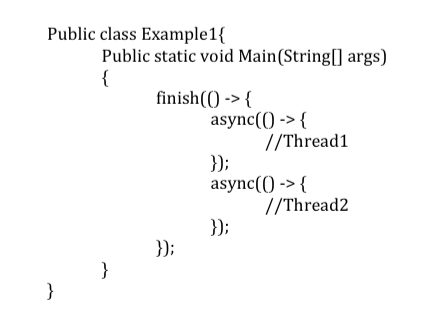
\includegraphics[scale=0.5]{../figs/Fig1.jpg} 
\end{figure}
\begin{figure}[h!]
  \caption{Computation Graph of the example program}
    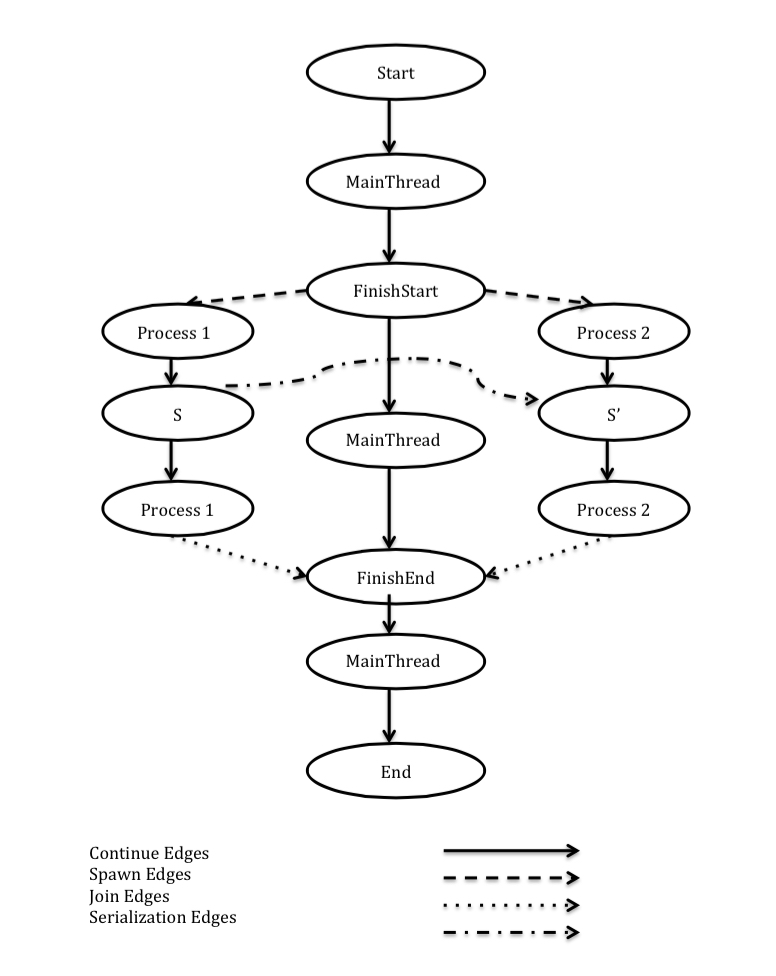
\includegraphics[scale=0.4]{../figs/Fig2.jpg}
\end{figure}

\subsubsection{Properties of Task Parallel Programs}
The following properties of task parallel programs can be verified using computation graphs.

\begin{enumerate}
\item
\textbf{Data Race:}
Data races occur in parallel programs when two or more tasks try to access shared variables such that at least one of the accesses is a 'write'. Data races cause the output of the program to become non-deterministic. 
\item
\textbf{Determinism:}
Determinism refers to obtaining the same result from a parallel program for a given input. There are different definitions that determine the degree of determinism in parallel programs.
\begin{enumerate}
\item
\textbf{Internal (or structural) determinism:\\}
This type of determinism requires the parallel program to not only produce the same output for a given input, but also to produce a unique computation graph for a given input. A program is internally deterministic only if it is free of data-races.
\item
\textbf{External (or functional) determinism:\\}
External determinism requires the parallel program to produce the same output when run on the same input. Program's executions for a given input may be different, but they ultimately produce the same output. In the presence of data-races, a program is externally deterministic if every pair of concurrent operators commute.
\end{enumerate}
\end{enumerate}

\subsection{Implementation details}
An HJ computation graph can be built using a tool called HJ-Viz. HJ-Viz processes the event logs produced by the HJLib runtime and generates a dot representation of the computation graph. The dot file can later be processed and displayed in the user's web browser using the HJ-Viz server. The drawback of this tool is that it does not store the computation graph in a logical data structure that can be traversed and analyzed to verify the properties of the program. Another drawback is that it does not save any memory references to objects. Hence, we need to create a tool that can build a computation graph of an HJ program during runtime and store the information in a logical data-structure that is easy to traverse and analyze.

The modified computation graph builder is implemented using Java Path Finder(JPF). It uses the Verification Runtime, specifically designed to run HJ programs using JPF. The HJ program is compiled using the VR and the class files are analyzed using JPF. JPF creates thread choice generators to systematically explore the state-space of the programs. We use one choice of thread interleavings at a time to observe the execution and build a computation graph for this execution. The VM listeners in JPF are extended to track the thread creations, executions, joins etc. Memory references are also registered in the computation graphs. The computation graphs are stored in DAG data structure. We are going to use jgrapht library that provides an implementation of this data structure.

Data races can be detected in a computation graph when two parallel nodes in the graph access a memory location and atleast one of the operations tries to modify it. A Topological traversal of the graph gives the order of execution of the various tasks. All the nodes that occur between  a pair of Finish-start and Finish-end nodes execute in parallel. The global memory accesses by these processes have to be checked and if conflicting memory-accesses are observed, then a data race should be reported.

For checking functional determinism of the program in the presence of data-races, JPF schedules on the memory location access that is part of the data race. If all the executions of the program produce the same result, then the program is functionally deterministic.

In programs with isolated regions (CG containing serialization edges), JPF creates schedules such that all possible orderings between the interfering isolated nodes is considered. The rest of the process for detecting data-races and checking determinism is carried out on all the obtained computation graphs.

\section{Validation}

Add stuff.



\section{Thesis Schedule}
The following schedule is an outline of submission dates for my Master's Thesis:

Submission to Advisor: February 8, 2016

Submission to Committee Members: February 22, 2016

Master's Thesis Defense: April 4, 2016


\bibliography{../bib/proposal}
\bibliographystyle{plain-annote}

\pagebreak

\begin{center}
\doublespacing

\textsc{Brigham Young University}

\textsc{Graduate Committee Approval}

of a thesis proposal submitted by

Eric S. Noonan
\end{center}

\noindent This thesis proposal has been read by each member of the
following graduate committee and by majority vote has been found to be
satisfactory.

\vspace{0.5cm}

\hrule

\vspace{0.5cm}

\newcommand{\signature}[1] {\vspace{1in} \noindent
\makebox[3.5in]{\hrulefill}  \hfill \makebox[2.5in]{\hrulefill}\\
\vspace{0.5cm} #1 \hfill Date \hspace{2in}}

\signature{Eric Mercer, Chair}

\signature{Jay McCarthy}

\signature{Mark Clement}

\signature{Quinn Snell, Graduate Coordinator}



\end{document} 
